\chapter{Concentratie en verdunning}\label{ch:g10:concentration-and-dilution}

Boven het bed van een patiënt hangt een infuuszak. Op het etiket staat
``0.9 \% natriumchloride'': zout in water, verder niets. Toch is het getal
0.9 geen detail. Te weinig zout, en de bloedcellen van de patiënt zouden
opzwellen met water; te veel, en ze zouden verschrompelen. Een oplossing
beschrijf je niet alleen met haar ingrediënten, maar met hoeveel \omterm{def:g6:solutions-and-solubility:solute}{opgeloste
stof} elk volume ervan bevat, haar concentratie. Dit hoofdstuk meet
concentraties, maakt oplossingen met een exacte concentratie, en verdunt
ze.

\begin{recall}
Een oplossing bestaat uit een \omterm{def:g6:solutions-and-solubility:solute}{oplosmiddel} en een of meer \omterm{def:g6:solutions-and-solubility:solute}{opgeloste
stoffen}; de \omterm{def:g6:solutions-and-solubility:solubility}{oplosbaarheid} is de grootste massa \omterm{def:g6:solutions-and-solubility:solute}{opgeloste stof} die een
gegeven hoeveelheid \omterm{def:g6:solutions-and-solubility:solute}{oplosmiddel} kan \omterm{def:g2:mixing-and-dissolving:dissolve}{oplossen}
(\cref{ch:g6:solutions-and-solubility}). De hoeveelheid van een stof is
$n = m/M$, in \omterm{def:g10:the-mole:amount}{mol} (\cref{ch:g10:the-mole}).
\end{recall}

\begin{omfigure}
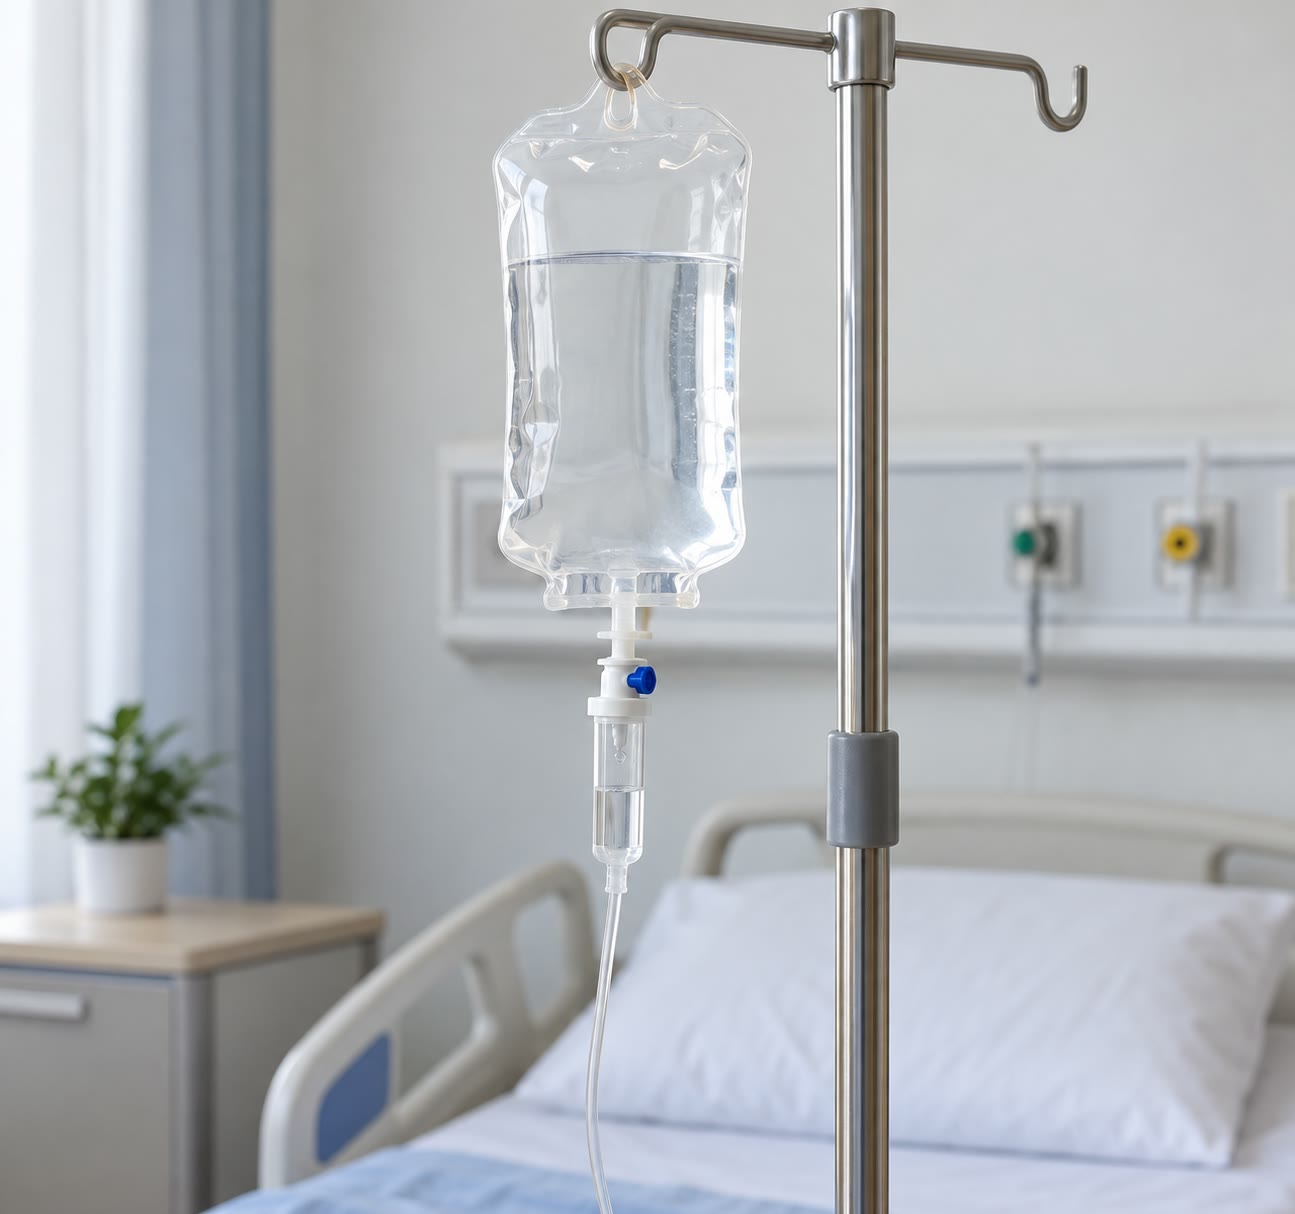
\includegraphics[width=0.42\linewidth]{images/book1/ai/g10-drip-bag.jpg}

{\small Een infuuszak met zoutoplossing: de concentratie moet kloppen.}
\end{omfigure}

\section{Massaconcentratie}

\begin{definition}[Massaconcentratie]\label{def:g10:concentration-and-dilution:mass-concentration}
De \emph{massaconcentratie}\index{massaconcentratie} $C_m$ van een
\omterm{def:g6:solutions-and-solubility:solute}{opgeloste stof} in een oplossing is de massa \omterm{def:g6:solutions-and-solubility:solute}{opgeloste stof} per volume
oplossing:
\[
  C_m = \frac{m_{\text{opgeloste stof}}}{V_{\text{oplossing}}},
\]
in gram per liter (\si{g/L}).
\end{definition}

\begin{example}[Suikerwater]\label{ex:g10:concentration-and-dilution:sugar}
Er wordt \qty{20}{g} suiker opgelost in water, en de oplossing wordt
aangevuld tot \qty{0.50}{L}. De \omterm{def:g10:concentration-and-dilution:mass-concentration}{massaconcentratie} van suiker is
$C_m = \qty{20}{g} / \qty{0.50}{L} = \qty{40}{g/L}$. Elk deel ervan heeft
dezelfde concentratie: een glas van \qty{0.20}{L} ervan bevat
$\qty{40}{g/L} \times \qty{0.20}{L} = \qty{8.0}{g}$ suiker.
\end{example}


\begin{remark}[Het volume is dat van de oplossing]\label{rem:g10:concentration-and-dilution:volume}
Het volume in $C_m$ is het volume van de hele oplossing, niet dat van het
water dat je erin giet: als een stof \omterm{def:g2:mixing-and-dissolving:dissolve}{oplost}, verandert het volume een
beetje. Daarom wordt een oplossing altijd \emph{aangevuld} tot een bekend
eindvolume, in een kolf met een maatstreep daarvoor.
\end{remark}

\begin{remark}[Concentratie is geen oplosbaarheid]\label{rem:g10:concentration-and-dilution:not-solubility}
% ledger: sol:NaCl, saline:NaCl
De \omterm{def:g6:solutions-and-solubility:solubility}{oplosbaarheid} van een stof is de \emph{grootste} concentratie die ze
kan bereiken; een oplossing kan elke concentratie hebben van nul tot die
grens. Natriumchloride lost bij \qty{25}{\celsius} op tot ongeveer
\qty{360}{g} per kilogram water; de infuuszak bevat maar \qty{9}{g} per
liter, heel ver van verzadiging.
\end{remark}

\begin{remark}[Percentages op etiketten]\label{rem:g10:concentration-and-dilution:percent}
% ledger: saline:NaCl
Op medische etiketten en etiketten van voedingsmiddelen betekent ``0.9
\%'' voor een vaste stof opgelost in water meestal \qty{0.9}{g} \omterm{def:g6:solutions-and-solubility:solute}{opgeloste
stof} per \qty{100}{mL} oplossing. In gram per liter is dat tien keer
zoveel: de infuuszak bevat \qty{9.0}{g/L} natriumchloride.
\end{remark}

\section{Molaire concentratie}

\begin{definition}[Molaire concentratie]\label{def:g10:concentration-and-dilution:molar-concentration}
De \emph{molaire concentratie}\index{molaire concentratie} $c$ van een
\omterm{def:g6:solutions-and-solubility:solute}{opgeloste stof} in een oplossing is de hoeveelheid \omterm{def:g6:solutions-and-solubility:solute}{opgeloste stof} per
volume oplossing:
\[
  c = \frac{n_{\text{opgeloste stof}}}{V_{\text{oplossing}}},
\]
in \omterm{def:g10:the-mole:amount}{mol} per liter (\si{mol/L}).
\end{definition}

\begin{proposition}[Van de ene concentratie naar de andere]\label{prop:g10:concentration-and-dilution:link}
Voor een \omterm{def:g6:solutions-and-solubility:solute}{opgeloste stof} met \omterm{def:g10:the-mole:molar-mass}{molaire massa} $M$ geldt
\[
  C_m = c \times M .
\]
\end{proposition}

\begin{proof}
$C_m = m / V = (n \times M) / V = (n / V) \times M = c \times M$.
\end{proof}

\begin{example}[De infuuszak in mol]\label{ex:g10:concentration-and-dilution:drip}
% ledger: saline:NaCl, saline:Na, aw:Na, aw:Cl
De infuuszak bevat \qty{9.0}{g/L} natriumchloride, met een \omterm{def:g10:the-mole:molar-mass}{molaire massa}
van \qty{58.5}{g/mol}. De \omterm{def:g10:concentration-and-dilution:molar-concentration}{molaire concentratie} is
\[
  c = \frac{C_m}{M} = \frac{\qty{9.0}{g/L}}{\qty{58.5}{g/mol}}
    = \qty{0.154}{mol/L}.
\]
Het etiket van de fabrikant geeft hetzelfde getal andersom: 154
duizendste \omterm{def:g10:the-mole:amount}{mol} natriumionen per liter.
\end{example}

\begin{remark}[Ionen in oplossing]\label{rem:g10:concentration-and-dilution:ions}
Natriumchloride \omterm{def:g2:mixing-and-dissolving:dissolve}{lost op} als losse \omterm{def:g9:ions:ion}{ionen} \ce{Na+} en \ce{Cl-}
(\cref{ch:g9:ions}): een oplossing van natriumchloride met
\qty{0.154}{mol/L} bevat \qty{0.154}{mol/L} natriumionen en
\qty{0.154}{mol/L} \omterm{def:g9:ions:ion}{chloride-ionen}. Hoe een ionaire vaste stof in water
uiteenvalt, is het onderwerp van een later hoofdstuk.
\end{remark}

\begin{omfigure}
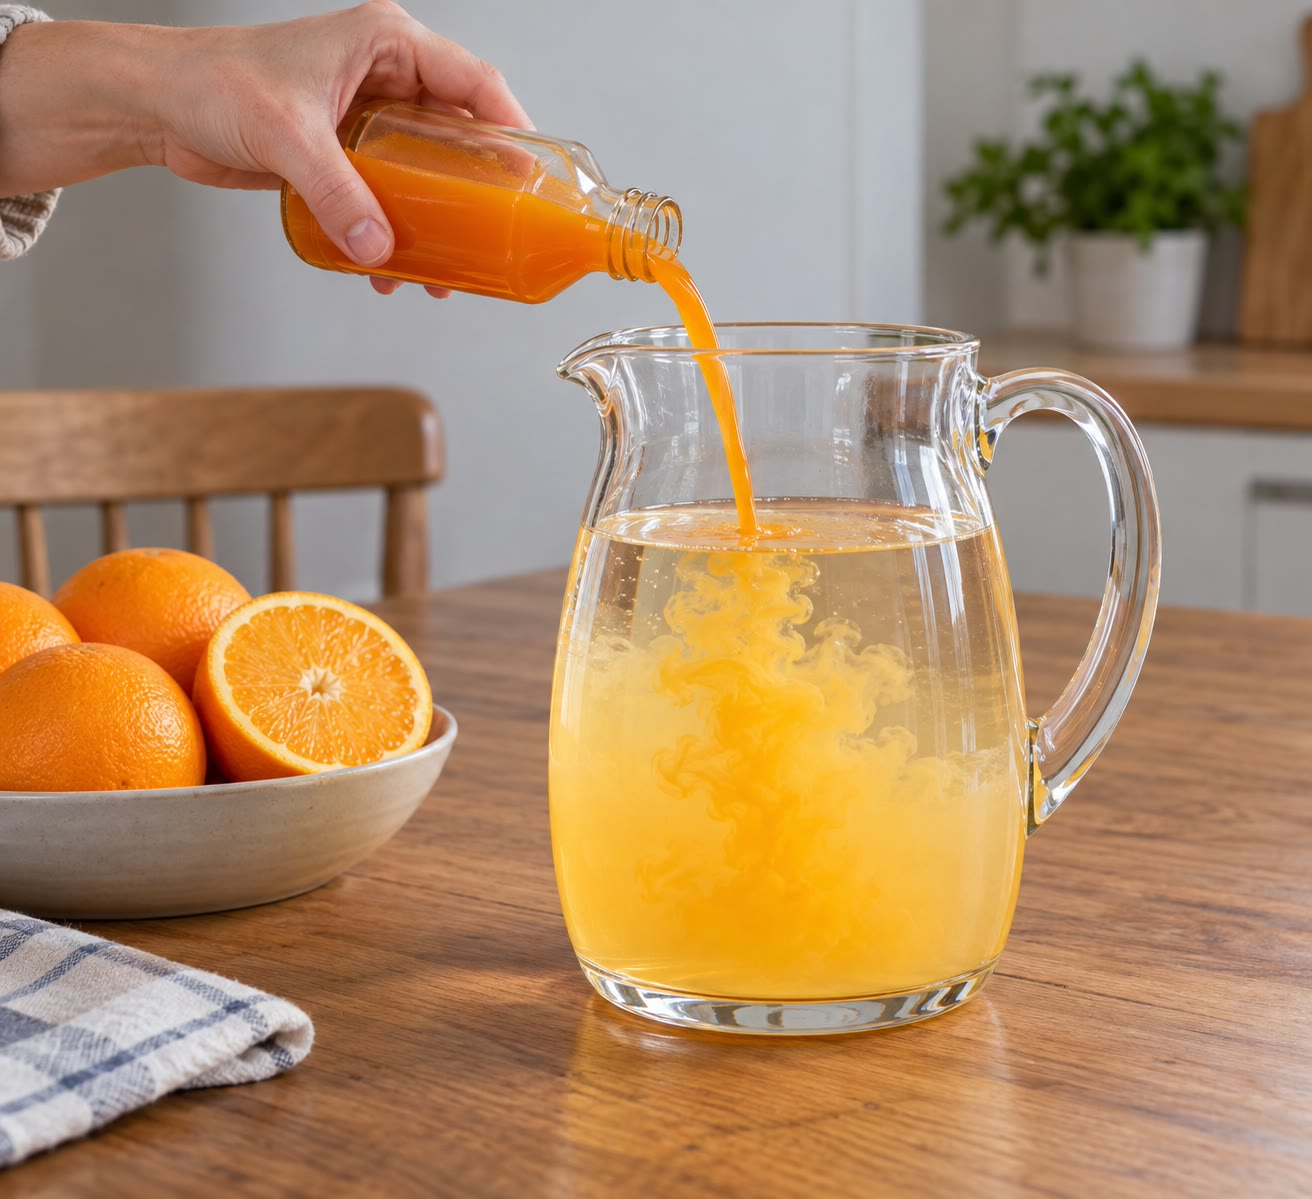
\includegraphics[width=0.45\linewidth]{images/book1/ai/g10-squash-jug.jpg}

{\small Ranja uit de fles wordt in een kan met water aangelengd: de drank
bevat dezelfde hoeveelheid vruchtensiroop, in een groter volume.}
\end{omfigure}

\section{Een oplossing maken door oplossen}

\begin{method}[Een oplossing maken door een vaste stof op te lossen]\label{met:g10:concentration-and-dilution:dissolving}
Om een volume $V$ oplossing met \omterm{def:g10:concentration-and-dilution:molar-concentration}{molaire concentratie} $c$ te maken:
\begin{enumerate}
  \item Bereken de benodigde hoeveelheid, $n = c \times V$, en de massa
        die je moet afwegen, $m = n \times M$.
  \item Weeg deze massa vaste stof af in een schaaltje op een balans.
  \item Giet de vaste stof via een trechter in een maatkolf met volume
        $V$; spoel het schaaltje en de trechter met gedestilleerd water na
        in de kolf, zodat er geen vaste stof verloren gaat.
  \item Vul met gedestilleerd water tot ongeveer de helft van de kolf en
        zwenk tot alle vaste stof is opgelost.
  \item Vul aan met gedestilleerd water tot de maatstreep, de laatste
        druppels met een druppelpipet; doe de stop erop en keer de kolf een
        paar keer om om te \omterm{def:g2:mixing-and-dissolving:mix}{mengen}.
\end{enumerate}
\end{method}

\begin{omfigure}
\begin{tikzpicture}[font=\small, scale=1.05]
  % 1. weigh
  \pic[transform shape] at (0,0) {balance};
  \fill[black!8, draw=black!55] (-0.45,0.8) -- (0.45,0.8) -- (0.38,0.98)
    -- (-0.38,0.98) -- cycle;
  \fill[white, draw=black!40] (-0.25,0.98) .. controls (-0.1,1.15) and
    (0.1,1.15) .. (0.25,0.98) -- cycle;
  \node[align=center, anchor=north] at (0,-0.2) {1. weeg\\ de vaste stof af};
  % 2. transfer through a funnel
  \pic[transform shape] at (3.2,0) {volflask={0.08}{omWater}};
  \pic[transform shape] at (3.2,3.0) {funnel};
  \draw[omProp, thick, -{Stealth}] (2.4,5.0) -- (2.85,4.65);
  \node[align=center, anchor=north] at (3.2,-0.2) {2. overbrengen,\\ naspoelen};
  % 3. half full, swirl
  \pic[transform shape] at (6.4,0) {volflask={0.45}{omWater}};
  \draw[omProp, thick, -{Stealth}] (5.55,0.5) arc[start angle=200,
    end angle=340, x radius=0.9, y radius=0.3];
  \node[align=center, anchor=north] at (6.4,-0.2) {3. half vol:\\ zwenken tot opgelost};
  % 4. to the mark
  \pic[transform shape] at (9.6,0) {volflask={1}{omWater}};
  \fill[black!45] (9.43,3.6) rectangle (9.77,3.85);
  \draw[omDef, thick, <-] (9.82,2.9) -- (10.6,3.3) node[right] {maatstreep};
  \node[align=center, anchor=north] at (9.6,-0.2) {4. vullen tot\\ de streep, stop\\
    erop en mengen};
\end{tikzpicture}

{\small Een oplossing maken door een vaste stof op te lossen: afwegen,
overbrengen, \omterm{def:g2:mixing-and-dissolving:dissolve}{oplossen}, en dan aanvullen tot de maatstreep van de
maatkolf.}
\end{omfigure}

\begin{inthelab}[Aanvullen tot de maatstreep]
De maatstreep van een maatkolf is een ring rond de hals. Water in een
smalle glazen buis eindigt niet vlak: het oppervlak buigt in het midden
naar beneden en vormt een meniscus. De kolf is vol als de
\emph{onderkant} van de meniscus de streep raakt, gezien met het oog op
de hoogte van de streep, zodat de voorkant en de achterkant van de ring
als één lijn te zien zijn. Van boven of van onder gezien kan het niveau
goed lijken terwijl het dat niet is.
\end{inthelab}

\begin{omfigure}
\begin{tikzpicture}[font=\small]
  \newcommand{\neck}[2]{% x, meniscus bottom height
    \fill[omWater] (#1-0.5,0) -- (#1-0.5,{#2+0.25}) .. controls
      (#1-0.25,#2) and (#1+0.25,#2) .. (#1+0.5,{#2+0.25}) -- (#1+0.5,0) -- cycle;
    \draw[black!60, line width=0.8pt] (#1-0.5,0) -- (#1-0.5,3);
    \draw[black!60, line width=0.8pt] (#1+0.5,0) -- (#1+0.5,3);
    \draw[omDef, line width=0.9pt] (#1-0.5,1.5) -- (#1+0.5,1.5);
    \draw[black!50] (#1-0.5,{#2+0.25}) .. controls (#1-0.25,#2) and
      (#1+0.25,#2) .. (#1+0.5,{#2+0.25});}
  \newcommand{\eye}[2]{% x, y: an eye looking to the right
    \draw[black!70] (#1-0.25,#2) .. controls (#1-0.1,#2+0.18) and
      (#1+0.1,#2+0.18) .. (#1+0.2,#2) .. controls (#1+0.1,#2-0.18) and
      (#1-0.1,#2-0.18) .. (#1-0.25,#2);
    \fill[black!70] (#1+0.05,#2) circle (0.06);}
  % right
  \neck{1.5}{1.5}
  \eye{-0.4}{1.5}
  \draw[dashed, black!50] (-0.1,1.5) -- (2.4,1.5);
  \node[align=center] at (1.5,-0.55) {goed: oog op hoogte,\\ onderkant op de streep};
  % too high
  \neck{6}{1.85}
  \eye{4.1}{1.85}
  \draw[dashed, black!50] (4.4,1.85) -- (6.9,1.85);
  \node[align=center] at (6,-0.55) {te veel water:\\ meniscus erboven};
  % too low
  \neck{10.5}{0.85}
  \eye{8.6}{0.85}
  \draw[dashed, black!50] (8.9,0.85) -- (11.4,0.85);
  \node[align=center] at (10.5,-0.55) {te weinig water:\\ meniscus eronder};
\end{tikzpicture}

{\small De hals van een maatkolf, vergroot en gezien met het oog op de
hoogte van de meniscus. De blauwe lijn is de maatstreep. Alleen de
linkerkolf is goed gevuld.}
\end{omfigure}

\section{Verdunnen}

\begin{definition}[Verdunning, stamoplossing, verdunningsfactor]\label{def:g10:concentration-and-dilution:dilution}
Een \emph{verdunning}\index{verdunning} verlaagt de concentratie van een
oplossing door \omterm{def:g6:solutions-and-solubility:solute}{oplosmiddel} toe te voegen. De geconcentreerde oplossing
waarmee je begint, is de \emph{stamoplossing}\index{stamoplossing}. De
\emph{verdunningsfactor}\index{verdunningsfactor} $F$ is de verhouding
van de concentratie van de stamoplossing tot die van de verdunde
oplossing:
\[
  F = \frac{c_{\text{stam}}}{c_{\text{verdund}}} .
\]
\end{definition}

\begin{proposition}[De hoeveelheid opgeloste stof blijft gelijk]\label{prop:g10:concentration-and-dilution:kept}
Bij een \omterm{def:g10:concentration-and-dilution:dilution}{verdunning} verandert de hoeveelheid \omterm{def:g6:solutions-and-solubility:solute}{opgeloste stof} niet: als een
volume $V_0$ \omterm{def:g10:concentration-and-dilution:dilution}{stamoplossing} met concentratie $c_0$ wordt aangevuld tot een
volume $V_1$, heeft de verdunde oplossing de concentratie $c_1$ die volgt
uit
\[
  c_0 \times V_0 = c_1 \times V_1,
  \qquad\text{dus}\qquad
  F = \frac{c_0}{c_1} = \frac{V_1}{V_0} .
\]
Hetzelfde geldt voor \omterm{def:g10:concentration-and-dilution:mass-concentration}{massaconcentraties}.
\end{proposition}

\begin{proof}
Er wordt alleen \omterm{def:g6:solutions-and-solubility:solute}{oplosmiddel} toegevoegd: de \omterm{def:g6:solutions-and-solubility:solute}{opgeloste stof} die met het
volume $V_0$ is meegenomen, een hoeveelheid $c_0 V_0$, zit helemaal in
het eindvolume $V_1$, waar ze de hoeveelheid $c_1 V_1$ vormt.
\end{proof}


\begin{method}[Een oplossing maken door verdunnen]\label{met:g10:concentration-and-dilution:diluting}
Om een volume $V_1$ oplossing met concentratie $c_1$ te maken uit een
\omterm{def:g10:concentration-and-dilution:dilution}{stamoplossing} met concentratie $c_0$:
\begin{enumerate}
  \item Bereken het volume \omterm{def:g10:concentration-and-dilution:dilution}{stamoplossing} dat je moet afnemen,
        $V_0 = c_1 V_1 / c_0$ (dus $V_1 / F$).
  \item Giet een beetje \omterm{def:g10:concentration-and-dilution:dilution}{stamoplossing} in een schoon bekerglas (pipetteer
        nooit rechtstreeks uit de fles) en neem precies $V_0$ af met een
        volumepipet, gevuld tot de maatstreep.
  \item Laat de pipet leeglopen in een maatkolf met volume $V_1$.
  \item Vul aan met gedestilleerd water tot de maatstreep, doe de stop
        erop en meng.
\end{enumerate}
\end{method}

\begin{example}[Een tienvoudige verdunning]\label{ex:g10:concentration-and-dilution:tenfold}
Een \omterm{def:g10:concentration-and-dilution:dilution}{stamoplossing} van kopersulfaat heeft $c_0 = \qty{0.10}{mol/L}$; er is
\qty{100.0}{mL} met $c_1 = \qty{0.010}{mol/L}$ nodig. De \omterm{def:g10:concentration-and-dilution:dilution}{verdunningsfactor}
is $F = 0.10 / 0.010 = 10$, dus $V_0 = \qty{100.0}{mL} / 10 =
\qty{10.0}{mL}$: een pipet van \qty{10.0}{mL} en een maatkolf van
\qty{100.0}{mL}.
\end{example}

\begin{omfigure}
\begin{tikzpicture}[font=\small, scale=0.85]
  % 1. take the stock with a pipette
  \pic[transform shape] at (0,0) {beaker={0.6}{cyan!70!blue!55}};
  \pic[transform shape] at (0,0.2) {pipette={1}{cyan!70!blue!55}};
  \node[align=center, anchor=north] at (0,-0.2) {1. pipetteer $V_0$\\ stamoplossing};
  \draw[omProp, very thick, -{Stealth}] (1.3,2.6) -- (2.6,2.6);
  % 2. empty it into the flask
  \pic[transform shape] at (4,0) {volflask={0.22}{cyan!70!blue!55}};
  \pic[transform shape] at (4,2.6) {pipette={0.12}{cyan!70!blue!55}};
  \node[align=center, anchor=north] at (4,-0.2) {2. laat leeglopen\\ in de kolf};
  \draw[omProp, very thick, -{Stealth}] (5.3,2.6) -- (6.6,2.6);
  % 3. water to the mark
  \pic[transform shape] at (8,0) {volflask={1}{cyan!70!blue!14}};
  \draw[omDef, thick, <-] (8.2,2.9) -- (9.1,3.4) node[right] {maatstreep};
  \node[align=center, anchor=north] at (8,-0.2) {3. water tot de streep:\\
    volume $V_1$};
\end{tikzpicture}

{\small Verdunnen: een volume $V_0$ \omterm{def:g10:concentration-and-dilution:dilution}{stamoplossing}, afgemeten met een pipet,
wordt in een maatkolf aangevuld tot $V_1$. De kleur vervaagt met de
\omterm{def:g10:concentration-and-dilution:dilution}{verdunningsfactor} $V_1 / V_0$.}
\end{omfigure}

\section{Een ijkreeks}

\begin{definition}[Standaardoplossing, ijkreeks]\label{def:g10:concentration-and-dilution:standard}
Een \emph{standaardoplossing}\index{standaardoplossing} is een oplossing
waarvan de concentratie nauwkeurig bekend is. Een
\emph{ijkreeks}\index{ijkreeks} is een reeks standaardoplossingen van
dezelfde \omterm{def:g6:solutions-and-solubility:solute}{opgeloste stof}, met toenemende concentraties, meestal gemaakt
door één \omterm{def:g10:concentration-and-dilution:dilution}{stamoplossing} te verdunnen; door een onbekende oplossing ermee
te vergelijken, schat je de concentratie van de onbekende.
\end{definition}

\begin{example}[Een blauwe reeks]\label{ex:g10:concentration-and-dilution:scale}
Uit een \omterm{def:g10:concentration-and-dilution:dilution}{stamoplossing} van kopersulfaat met \qty{0.20}{mol/L} worden zes
\omterm{def:g10:concentration-and-dilution:standard}{standaardoplossingen} gemaakt met 0.02, 0.04, 0.06, 0.08, 0.10 en
\qty{0.12}{mol/L}, elk in gelijke buizen, tot dezelfde hoogte gevuld. Een
oplossing met een onbekende concentratie, in eenzelfde buis, is donkerder
dan de buis met \qty{0.06}{mol/L} en lichter dan die met
\qty{0.08}{mol/L}: haar concentratie ligt daartussen, ongeveer
\qty{0.07}{mol/L}.
\end{example}

\begin{omfigure}
\begin{tikzpicture}[font=\small]
  \foreach \i/\c/\p in {0/0.02/8, 1/0.04/16, 2/0.06/24, 3/0.08/32,
                        4/0.10/40, 5/0.12/48} {
    \pic at (1.2*\i,0) {testtube={0.75}{cyan!70!blue!\p}};
    \node[anchor=north] at (1.2*\i,-0.15) {\c};
  }
  \pic at (8.4,0) {testtube={0.75}{cyan!70!blue!28}};
  \node[anchor=north] at (8.4,-0.15) {?};
  \draw[black!40] (7.55,-0.6) -- (7.55,3.2);
  \node[anchor=north] at (3,-0.7) {concentratie (\si{mol/L})};
  \node[anchor=north] at (8.4,-0.7) {onbekend};
\end{tikzpicture}

{\small Een \omterm{def:g10:concentration-and-dilution:standard}{ijkreeks} van kopersulfaatoplossingen en een onbekende
oplossing. De onbekende ligt tussen de derde en de vierde buis.}
\end{omfigure}

\begin{safety}{\ghs[0.82cm]{GHS05}\ghs[0.82cm]{GHS07}\ghs[0.82cm]{GHS09}}
% ledger: ghs:CuSO4
Kopersulfaatoplossingen: schadelijk bij inslikken, irriterend voor de
huid, schadelijk voor de ogen, zeer giftig voor in het water levende
organismen. Veiligheidsbril en handschoenen; de gebruikte oplossingen
worden ingezameld voor verwerking, nooit door de gootsteen gespoeld.
\end{safety}

\begin{remark}[De grenzen van het oog]\label{rem:g10:concentration-and-dilution:eye}
Het oog kan alleen zeggen ``tussen deze twee buizen''. Om een
concentratie preciezer te meten uit de kleur van een oplossing, meten
scheikundigen hoeveel licht die opneemt; een later hoofdstuk doet precies
dat.
\end{remark}

\section{Oefeningen}

\begin{exercise}[$\star$]\label{exo:g10:concentration-and-dilution:1}
Er wordt \qty{5.0}{g} suiker opgelost tot \qty{250}{mL} oplossing.
Bereken de \omterm{def:g10:concentration-and-dilution:mass-concentration}{massaconcentratie} van suiker in gram per liter.
\end{exercise}

\begin{exercise}[$\star$]\label{exo:g10:concentration-and-dilution:2}
Een oplossing van \qty{200}{mL} bevat \qty{0.050}{mol} glucose. Bereken
de \omterm{def:g10:concentration-and-dilution:molar-concentration}{molaire concentratie}.
\end{exercise}

\begin{exercise}[$\star$]\label{exo:g10:concentration-and-dilution:3}
Hoeveel watervrij kopersulfaat \ce{CuSO4} moet je afwegen om
\qty{100.0}{mL} oplossing met \qty{0.10}{mol/L} te maken?
\end{exercise}

\begin{exercise}[$\star$]\label{exo:g10:concentration-and-dilution:4}
Een \omterm{def:g10:concentration-and-dilution:dilution}{stamoplossing} met \qty{1.0}{mol/L} wordt verdund tot
\qty{0.050}{mol/L}. Wat is de \omterm{def:g10:concentration-and-dilution:dilution}{verdunningsfactor}? Hoeveel \omterm{def:g10:concentration-and-dilution:dilution}{stamoplossing}
is er nodig voor \qty{100.0}{mL} verdunde oplossing?
\end{exercise}

\begin{exercise}[$\star$]\label{exo:g10:concentration-and-dilution:5}
Een oplossing van natriumchloride heeft een \omterm{def:g10:concentration-and-dilution:molar-concentration}{molaire concentratie} van
\qty{0.10}{mol/L}. Wat is haar \omterm{def:g10:concentration-and-dilution:mass-concentration}{massaconcentratie}?
\end{exercise}

\begin{exercise}[$\star\star$]\label{exo:g10:concentration-and-dilution:6}
Hoeveel van een \omterm{def:g10:concentration-and-dilution:dilution}{stamoplossing} met \qty{0.50}{mol/L} moet je afnemen om
\qty{250.0}{mL} oplossing met \qty{0.020}{mol/L} te maken? Noem de twee
stukken glaswerk die je gebruikt.
\end{exercise}

\begin{exercise}[$\star\star$]\label{exo:g10:concentration-and-dilution:7}
Waarom maak je een oplossing met een exacte concentratie in een maatkolf
en niet in een bekerglas met een schaalverdeling? Waarom meet je een
volume \omterm{def:g10:concentration-and-dilution:dilution}{stamoplossing} af met een volumepipet en niet met een maatcilinder?
\end{exercise}

\begin{exercise}[$\star\star$]\label{exo:g10:concentration-and-dilution:8}
Kijk naar de \omterm{def:g10:concentration-and-dilution:standard}{ijkreeks} van kopersulfaat. Een tweede onbekende is lichter
dan de buis met \qty{0.04}{mol/L} maar donkerder dan die met
\qty{0.02}{mol/L}. Schat de concentratie. Hoe zou je de reeks kunnen
aanpassen om haar preciezer te schatten?
\end{exercise}

\begin{exercise}[$\star\star$]\label{exo:g10:concentration-and-dilution:9}
Een glucoseoplossing voor een infuus bevat \qty{50}{g/L} glucose
\ce{C6H12O6}. Bereken de \omterm{def:g10:concentration-and-dilution:molar-concentration}{molaire concentratie}.
\end{exercise}

\begin{exercise}[$\star\star$]\label{exo:g10:concentration-and-dilution:10}
Een siroop wordt gemaakt door \qty{342}{g} sacharose \ce{C12H22O11} op
te lossen tot \qty{1.00}{L} oplossing. Bereken de \omterm{def:g10:concentration-and-dilution:molar-concentration}{molaire concentratie}.
De siroop wordt daarna tien keer verdund. Hoeveel sacharose bevat een
lepel van \qty{20}{mL} van de verdunde siroop?
\end{exercise}

\begin{exercise}[$\star\star$]\label{exo:g10:concentration-and-dilution:11}
Een oplossing heeft een \omterm{def:g10:concentration-and-dilution:mass-concentration}{massaconcentratie} van \qty{12}{g/L}. Wat is de
concentratie (a) nadat er water is toegevoegd zodat het volume
verdubbelt; (b) nadat de helft van het water is verdampt, terwijl alle
\omterm{def:g6:solutions-and-solubility:solute}{opgeloste stof} opgelost blijft?
\end{exercise}

\begin{exercise}[$\star\star\star$]\label{exo:g10:concentration-and-dilution:12}
Een oplossing met \qty{0.10}{mol/L} wordt tien keer verdund, het
resultaat nog eens tien keer, en daarna nog een keer.
\begin{enumerate}
  \item Wat is de eindconcentratie?
  \item Waarom doe je dit in drie stappen en niet in één \omterm{def:g10:concentration-and-dilution:dilution}{verdunning} met
        een factor 1000 (denk aan de volumes van het benodigde glaswerk)?
\end{enumerate}
\end{exercise}

\begin{exercise}[$\star\star\star$]\label{exo:g10:concentration-and-dilution:13}
Er wordt \qty{11.1}{g} calciumchloride \ce{CaCl2} opgelost tot
\qty{500.0}{mL} oplossing. In water valt de vaste stof uiteen in
calciumionen \ce{Ca^2+} en \omterm{def:g9:ions:ion}{chloride-ionen} \ce{Cl-}.
\begin{enumerate}
  \item Bereken de \omterm{def:g10:concentration-and-dilution:molar-concentration}{molaire concentratie} van het opgeloste
        calciumchloride.
  \item Leid daaruit de \omterm{def:g10:concentration-and-dilution:molar-concentration}{molaire concentraties} van de calciumionen en van
        de \omterm{def:g9:ions:ion}{chloride-ionen} in de oplossing af.
\end{enumerate}
\end{exercise}

\begin{exercise}[$\star\star\star$]\label{exo:g10:concentration-and-dilution:14}
Een maatkolf van \qty{100.0}{mL} heeft een hals met een binnendiameter
van \qty{1.2}{cm}. Een leerling vult hem zo dat de onderkant van de
meniscus \qty{2}{mm} boven de maatstreep staat.
\begin{enumerate}
  \item Hoeveel water is er te veel toegevoegd (volume van een cilinder:
        $\pi r^2 h$)?
  \item Met welk percentage is de concentratie van de oplossing te laag?
\end{enumerate}
\end{exercise}

\begin{exercise}[$\star\star\star$]\label{exo:g10:concentration-and-dilution:15}
Er wordt \qty{100}{mL} natriumchlorideoplossing met \qty{0.20}{mol/L}
gemengd met \qty{300}{mL} natriumchlorideoplossing met
\qty{0.10}{mol/L}. Bereken de concentratie van het \omterm{def:g6:pure-substances-and-mixtures:mixture}{mengsel}, aangenomen
dat de volumes optellen. Is het het gemiddelde van de twee
concentraties? Leg uit.
\end{exercise}

\section{Probleem: De infuuszak}

\begin{problem}[{Weekendprobleem --- hoeveel van een geconcentreerde
zoutoplossing gaat er in één zak ``0.9 \%'' fysiologisch zout?}]
\label{pb:g10:concentration-and-dilution:1}
% ledger: saline:NaCl, saline:Na, sol:NaCl, aw:Na, aw:Cl, const:NA
Het laboratorium van een ziekenhuisapotheek heeft een geconcentreerde,
steriele oplossing van natriumchloride met \qty{200}{g/L} (op het
etiket: ``20 \%''). Het moet zakken van \qty{500}{mL} van de ``0.9 \%''
oplossing voor infusen maken, door de geconcentreerde oplossing te
verdunnen met steriel water.

\medskip
\noindent\textbf{Deel I --- Wat 0.9 \% betekent.}
\begin{enumerate}
  \item Het etiket ``0.9 \%'' betekent \qty{0.9}{g} zout per
        \qty{100}{mL} oplossing. Geef de \omterm{def:g10:concentration-and-dilution:mass-concentration}{massaconcentratie} in \si{g/L}.
  \item Druk haar ook uit in milligram per milliliter.
  \item Hoeveel natriumchloride bevat een zak van \qty{500}{mL}?
  \item Natriumchloride \omterm{def:g2:mixing-and-dissolving:dissolve}{lost op} tot ongeveer \qty{360}{g} per kilogram
        water. Is de oplossing in de zak ver van verzadiging?
  \item Een patiënt krijgt per dag \qty{1.0}{L} van deze oplossing.
        Hoeveel zout is dat?
\end{enumerate}

\medskip
\noindent\textbf{Deel II --- In \omterm{def:g10:the-mole:amount}{mol}.}
\begin{enumerate}[resume]
  \item Bereken de \omterm{def:g10:the-mole:molar-mass}{molaire massa} van natriumchloride.
  \item Bereken de \omterm{def:g10:concentration-and-dilution:molar-concentration}{molaire concentratie} van de oplossing in de zak.
  \item Welke hoeveelheid natriumchloride bevat één zak?
  \item Wat zijn de \omterm{def:g10:concentration-and-dilution:molar-concentration}{molaire concentraties} van natriumionen en van
        \omterm{def:g9:ions:ion}{chloride-ionen} in de zak?
  \item Hoeveel natriumionen bevat één zak?
\end{enumerate}

\medskip
\noindent\textbf{Deel III --- Uit de geconcentreerde oplossing.}
\begin{enumerate}[resume]
  \item Bereken de \omterm{def:g10:concentration-and-dilution:dilution}{verdunningsfactor} tussen de geconcentreerde oplossing en
        de oplossing in de zak.
  \item Hoeveel natriumchloride moet er voor één zak uit de geconcentreerde
        oplossing komen? Leid daaruit af hoeveel geconcentreerde oplossing
        je moet afnemen.
  \item Controleer dit volume met de \omterm{def:g10:concentration-and-dilution:dilution}{verdunningsfactor}.
  \item Bereken de \omterm{def:g10:concentration-and-dilution:molar-concentration}{molaire concentratie} van de geconcentreerde oplossing,
        en controleer dat $c_0 V_0 = c_1 V_1$.
  \item Hoeveel steriel water wordt er dan ongeveer toegevoegd (neem aan
        dat de volumes optellen)?
\end{enumerate}

\medskip
\noindent\textbf{Deel IV --- Glaswerk en nauwkeurigheid.}
\begin{enumerate}[resume]
  \item Er bestaat geen volumepipet van dit volume. Welk stuk glaswerk,
        met een schaalverdeling in tienden van een milliliter, zou het
        kunnen afmeten?
  \item In welk vat moet het eindvolume aangevuld worden om nauwkeurig te
        zijn?
  \item Als er \qty{23.0}{mL} afgenomen werd in plaats van het juiste
        volume, welke \omterm{def:g10:concentration-and-dilution:mass-concentration}{massaconcentratie} zou de zak dan hebben? Met welk
        percentage zou die afwijken?
  \item Geef het eindantwoord: hoeveel van de geconcentreerde oplossing
        gaat er in één zak van \qty{500}{mL}?
\end{enumerate}
\end{problem}
